% Transcribed saved root-bootstrap estimates; provenance in evidence_data.json.
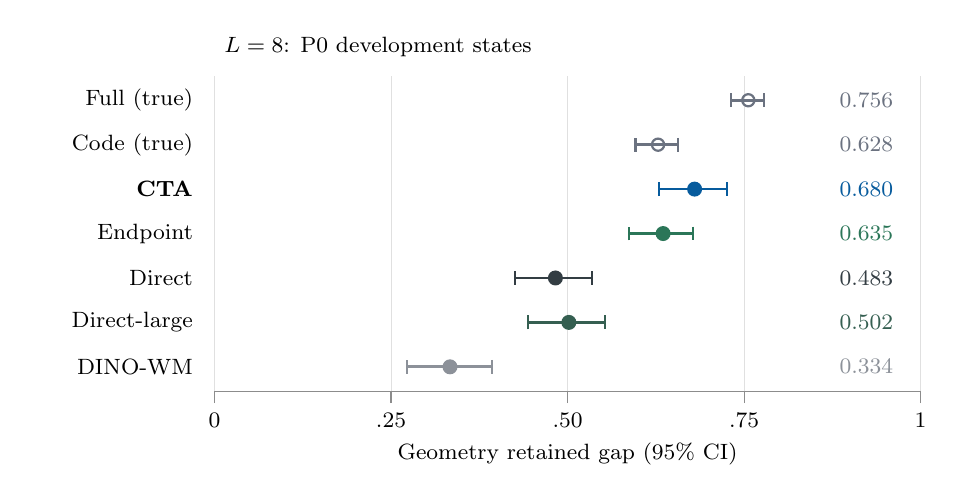
\begin{tikzpicture}
\definecolor{ctaplotblue}{HTML}{075B9D}
\definecolor{ctaplotgreen}{HTML}{2B7658}
\definecolor{ctaplotdeepgreen}{HTML}{355F51}
\definecolor{ctaplotdark}{HTML}{333D43}
\definecolor{ctaplotpriv}{HTML}{6B7280}
\definecolor{ctaplotdino}{HTML}{8C9199}
\begin{axis}[
  width=0.87\linewidth,
  height=2.20in,
  xmin=0, xmax=1,
  ymin=0.45, ymax=7.55,
  xtick={0,0.25,0.5,0.75,1},
  xticklabels={0,.25,.50,.75,1},
  ytick={7,6,5,4,3,2,1},
  yticklabels={Full (true),Code (true),\textbf{CTA},Endpoint,Direct,Direct-large,DINO-WM},
  font=\fontsize{8}{9}\selectfont,
  tick label style={font=\fontsize{8}{9}\selectfont},
  yticklabel style={text width=0.78in,align=right},
  xlabel={Geometry retained gap (95\% CI)},
  xlabel style={font=\fontsize{8}{9}\selectfont,yshift=1pt},
  axis x line*=bottom,
  axis y line*=left,
  y axis line style={draw=none},
  axis line style={black!45,line width=0.4pt},
  tick align=outside,
  tick style={black!45,line width=0.4pt},
  ytick style={draw=none},
  xmajorgrids=true,
  grid style={black!12,line width=0.3pt},
  clip=false,
  enlarge y limits=false,
]
\node[anchor=south west,font=\fontsize{8}{9}\selectfont]
  at (rel axis cs:0,1.03) {$L=8$: P0 development states};
\addplot[
  only marks,mark=o,mark options={fill=white,line width=0.8pt},mark size=2.2pt,color=ctaplotpriv,line width=1.0pt,
  error bars/.cd,x dir=both,x explicit,
  error bar style={line width=1.0pt},
  error mark options={rotate=90,mark size=2.5pt,line width=0.8pt}
] coordinates {(0.756003,7) +=(0.022116,0) -=(0.024909,0)};
\node[anchor=east,text=ctaplotpriv,font=\fontsize{8}{9}\selectfont]
  at (axis cs:0.975,7) {0.756};
\addplot[
  only marks,mark=o,mark options={fill=white,line width=0.8pt},mark size=2.2pt,color=ctaplotpriv,line width=1.0pt,
  error bars/.cd,x dir=both,x explicit,
  error bar style={line width=1.0pt},
  error mark options={rotate=90,mark size=2.5pt,line width=0.8pt}
] coordinates {(0.628188,6) +=(0.028753,0) -=(0.031862,0)};
\node[anchor=east,text=ctaplotpriv,font=\fontsize{8}{9}\selectfont]
  at (axis cs:0.975,6) {0.628};
\addplot[
  only marks,mark=*,mark size=2.2pt,color=ctaplotblue,line width=1.0pt,
  error bars/.cd,x dir=both,x explicit,
  error bar style={line width=1.0pt},
  error mark options={rotate=90,mark size=2.5pt,line width=0.8pt}
] coordinates {(0.679928,5) +=(0.045792,0) -=(0.050448,0)};
\node[anchor=east,text=ctaplotblue,font=\fontsize{8}{9}\selectfont]
  at (axis cs:0.975,5) {0.680};
\addplot[
  only marks,mark=*,mark size=2.2pt,color=ctaplotgreen,line width=1.0pt,
  error bars/.cd,x dir=both,x explicit,
  error bar style={line width=1.0pt},
  error mark options={rotate=90,mark size=2.5pt,line width=0.8pt}
] coordinates {(0.635334,4) +=(0.042480,0) -=(0.047753,0)};
\node[anchor=east,text=ctaplotgreen,font=\fontsize{8}{9}\selectfont]
  at (axis cs:0.975,4) {0.635};
\addplot[
  only marks,mark=*,mark size=2.2pt,color=ctaplotdark,line width=1.0pt,
  error bars/.cd,x dir=both,x explicit,
  error bar style={line width=1.0pt},
  error mark options={rotate=90,mark size=2.5pt,line width=0.8pt}
] coordinates {(0.482833,3) +=(0.052255,0) -=(0.057436,0)};
\node[anchor=east,text=ctaplotdark,font=\fontsize{8}{9}\selectfont]
  at (axis cs:0.975,3) {0.483};
\addplot[
  only marks,mark=*,mark size=2.2pt,color=ctaplotdeepgreen,line width=1.0pt,
  error bars/.cd,x dir=both,x explicit,
  error bar style={line width=1.0pt},
  error mark options={rotate=90,mark size=2.5pt,line width=0.8pt}
] coordinates {(0.501882,2) +=(0.051130,0) -=(0.057361,0)};
\node[anchor=east,text=ctaplotdeepgreen,font=\fontsize{8}{9}\selectfont]
  at (axis cs:0.975,2) {0.502};
\addplot[
  only marks,mark=*,mark size=2.2pt,color=ctaplotdino,line width=1.0pt,
  error bars/.cd,x dir=both,x explicit,
  error bar style={line width=1.0pt},
  error mark options={rotate=90,mark size=2.5pt,line width=0.8pt}
] coordinates {(0.333532,1) +=(0.059297,0) -=(0.061128,0)};
\node[anchor=east,text=ctaplotdino,font=\fontsize{8}{9}\selectfont]
  at (axis cs:0.975,1) {0.334};
\end{axis}
\end{tikzpicture}
